\begin{refsection}

\chapter{Rb--Sr, Sm--Nd, Lu--Hf and Re--Os}\label{ch:PD-R}

\noindent\begin{minipage}[t]{.3\linewidth}
\strut\vspace*{-\baselineskip}\newline
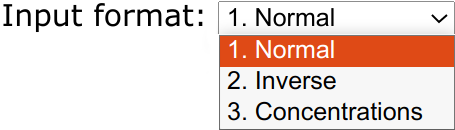
\includegraphics[width=\linewidth]{../figures/PDformats.png}
\end{minipage}
\begin{minipage}[t]{.7\textwidth}
  Simple parent-daughter chronometers can be specified in three
  different input formats. See Chapter~\ref{ch:PD} for details.
\end{minipage}

\begin{script}
RbSr <- read.data('RbSr1.csv',method='Rb-Sr',format=1)
SmNd <- read.data('SmNd2.csv',method='Sm-Nd',format=2)
LuHf <- read.data('LuHf3.csv',method='Lu-Hf',format=3)
ReOs <- read.data('ReOs2.csv',method='Re-Os',format=2)
\end{script}

\noindent which returns lists with items \texttt{format} and
\texttt{x} containing the input format and isotopic ratio data,
respectively.\\

\noindent\begin{minipage}[t]{.15\linewidth}
\strut\vspace*{-\baselineskip}\newline
\includegraphics[width=\linewidth]{../figures/PbPbPlotdevices.png}\\
\end{minipage}
\begin{minipage}[t]{.85\textwidth}
  The simple parent daughter chronometers can be visualised on the
  same five plot devices as the Pb--Pb, Th--Pb and K--Ca methods.
  Additionally, the single aliquot age estimates can also be reported
  in a downloadable data table.
\end{minipage}

\section{Stable isotope ratios and decay constants}\label{sec:PD-Lambda}

\noindent\begin{minipage}[t]{.6\linewidth}
\strut\vspace*{-\baselineskip}\newline
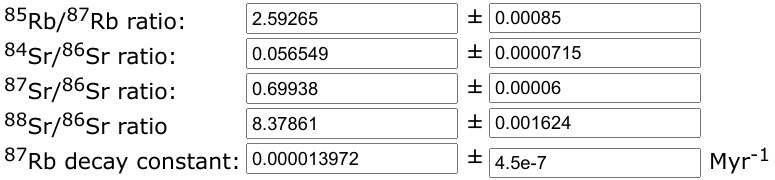
\includegraphics[width=\linewidth]{../figures/RbSrLambda.png}
\end{minipage}
\begin{minipage}[t]{.4\linewidth}
The default \textsuperscript{85}Rb/\textsuperscript{87}Rb ratio is
given by \citet{catanzaro1969}, and the
\textsuperscript{84}Sr/\textsuperscript{86}Sr and
\textsuperscript{88}Sr/\textsuperscript{87}Sr-ratios by
\citet{moore1982}. The default value for the non-radiogenic
\textsuperscript{87}Sr/\textsuperscript{86}Rb ratio is taken from
\citet{compston1971}. The latter value can, of course, be replaced by
the isochron intercept in all the plotting functions. The
\textsuperscript{87}Rb decay constant is given by \citet{villa2015}.
\end{minipage}

\begin{script}
# change the decay constant to the Steiger and Jaeger (1977) value:
settings('lambda','Rb87',0.0000142,0)
\end{script}

\noindent\begin{minipage}[t]{.6\linewidth}
\strut\vspace*{-\baselineskip}\newline
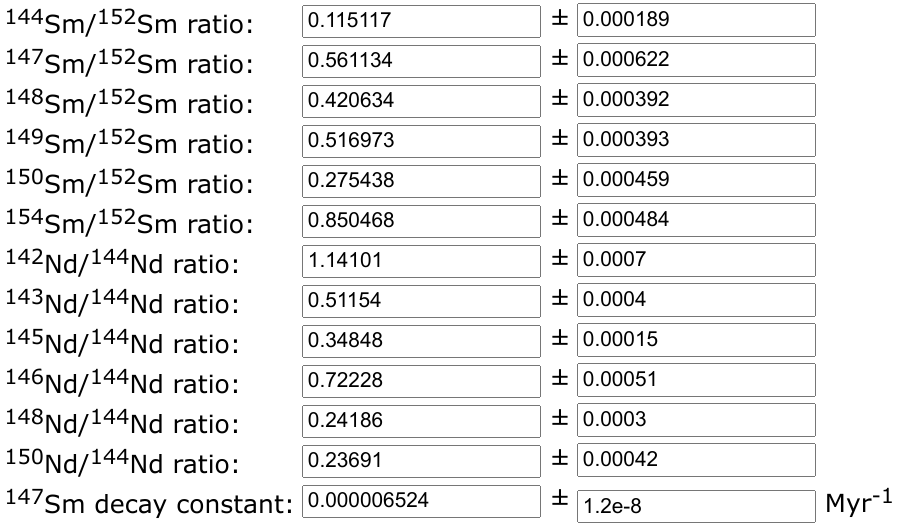
\includegraphics[width=\linewidth]{../figures/SmNdLambda.png}
\end{minipage}
\begin{minipage}[t]{.4\linewidth}
  The default isotopic compositions of Sm and Nd were taken from
  \citet{chang2002} and \citet{zhao2005}, respectively. The
  \textsuperscript{147}Sm decay constant is given by
  \citet{lugmair1978}.
\end{minipage}

\begin{script}
# change the decay constant to the Lugmair and Marti (1978) value:
settings('lambda','Sm147',0.000006540,0.000000049)
\end{script}

\noindent\begin{minipage}[t]{.6\linewidth}
\strut\vspace*{-\baselineskip}\newline
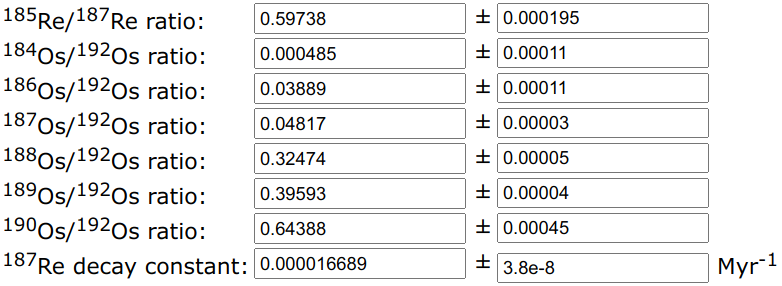
\includegraphics[width=\linewidth]{../figures/ReOsLambda.png}
\end{minipage}
\begin{minipage}[t]{.4\linewidth}
The default \textsuperscript{185}Re/\textsuperscript{187}Re ratio is
given by \citet{gramlich1973}, and the Os isotopic composition from
\citet{volkening1991}. The \textsuperscript{187}Re decay constant is
given by \citet{smoliar1996}.\\
\end{minipage}

\begin{script}
# change the decay constant to the Selby et al. (2007) value:
settings('lambda','Re187',0.000016689,0.000000038)
\end{script}

\noindent\begin{minipage}[t]{.6\linewidth}
\strut\vspace*{-\baselineskip}\newline
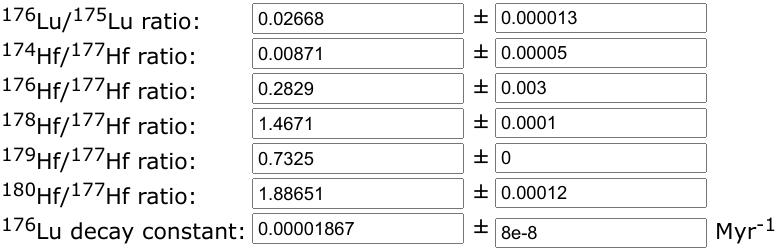
\includegraphics[width=\linewidth]{../figures/LuHfLambda.png}
\end{minipage}
\begin{minipage}[t]{.4\linewidth}
The default \textsuperscript{176}Lu/\textsuperscript{175}Lu ratio is
given by \citet{delaeter2006}, and the non-radiogenic Hf-composition
by \citet{patchett1983}. The \textsuperscript{176}Lu decay constant is
given by \citet{soderlund2004}.
\end{minipage}

\begin{script}
# change the decay constant to the Scherer et al. (2001) value:
settings('lambda','Lu176',0.00001865,0.00000015)
\end{script}

\section{Isochrons}\label{sec:PDisochrons}

\begin{enumerate}

\item\noindent\begin{minipage}[t]{.45\linewidth}
\strut\vspace*{-\baselineskip}\newline
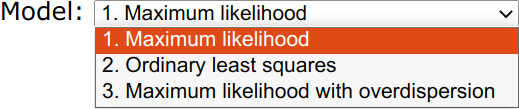
\includegraphics[width=\linewidth]{../figures/PbPbIsochronModels.png}
\end{minipage}
\begin{minipage}[t]{.55\linewidth}
  As with all the other chronometers, isochrons can be fitted using
  three algorithms, which represent three different ways to handle
  overdispersion.
\end{minipage}

\begin{script}
isochron(RbSr,model=1) # York regression
isochron(SmNd,model=2) # ordinary least squares regression
isochron(LuHf,model=3) # maximum likelihood fit with overdispersion
\end{script}

\item\noindent\begin{minipage}[t]{.22\linewidth}
  \strut\vspace*{-1.2\baselineskip}\newline
  
\includegraphics[width=\linewidth]{../figures/PbPbisochronInverse.png}
\end{minipage}
  \begin{minipage}[t]{.78\linewidth}
    Data can be fitted using conventional or inverse isochrons
    (Section~\ref{sec:inverseIsochrons}).
\end{minipage}

If P is the radioactive parent, D is the radiogenic daughter, and d is
a non-radiogenic isotope of the daughter element, then the
conventional isochron plots D/d vs. P/d, and the inverse isochron
plots d/D vs. P/D. For example, using the CLI:
  
\begin{script}
isochron(ReOs,inverse=FALSE) # 187Os/188Os vs. 187Re/188Os
isochron(ReOs,inverse=TRUE)  # 188Os/187Os vs. 187Re/187Os
\end{script}

\item\noindent\begin{minipage}[t]{.4\linewidth}
\strut\vspace*{-\baselineskip}\newline

\includegraphics[width=\linewidth]{../figures/concordiaexterr.png}
\end{minipage}
\begin{minipage}[t]{.6\linewidth}
  Ticking the box adds the decay constant error to the isochron age
  uncertainty.
\end{minipage}

\item All the other options are the same as the generic regression
  function of Section~\ref{sec:OtherRegression}.

\end{enumerate}

\section{Ages, weighted means, radial, KDE and CAD plots}\label{sec:PDages}

\begin{enumerate}

\item\noindent\begin{minipage}[t]{.5\linewidth}
\strut\vspace*{-\baselineskip}\newline
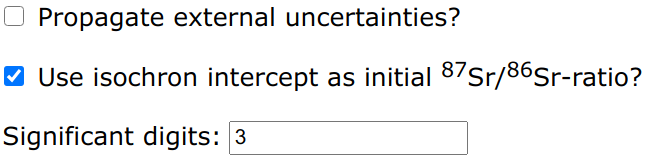
\includegraphics[width=\linewidth]{../figures/PDages.png}
\end{minipage}
\begin{minipage}[t]{.5\linewidth}
  The ages of individual aliquots can be tabulated either with or
  without decay constant uncertainties, using either a nominal
  inherited daughter component or an isochron-derived initial ratio.
\end{minipage}

\begin{console}
age(RbSr,exterr=FALSE,i2i=TRUE,sigdig=3)
\end{console}

\item\noindent\begin{minipage}[t]{.55\linewidth}
\strut\vspace*{-\baselineskip}\newline
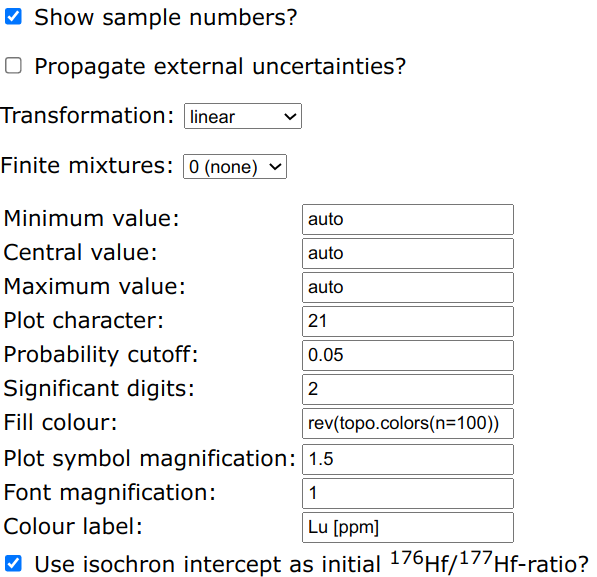
\includegraphics[width=\linewidth]{../figures/LuHfRadial.png}
\end{minipage}
\begin{minipage}[t]{.45\linewidth}
  The single aliquot ages can be plotted on radial plots, using all
  the same options as mentioned in Sections~\ref{sec:OtherRadial},
  \ref{sec:UPbRadial}, \ref{sec:ThPbPbOtherPlots} and
  \ref{sec:ArArKCaOtherPlots}. In this example, six numbered Lu--Hf
  aliquots are plotted on a linear scale and colour-coded according to
  the Lu concentration, which is specified in the optional
  \texttt{(C)} column in the input table (not shown), an using an
  inverted topographic colour ramp.  Plot symbols are magnified by a
  factor of 1.5. All other settings follow the default settings.
\end{minipage}

\begin{script}
radialplot(LuHf,show.numbers=TRUE,transformation='linear',cex=1.5,
           levels=LuHf$x[,'Lu'],bg=rev(topo.colors(n=100)),i2i=TRUE)
\end{script}

\item\noindent\begin{minipage}[t]{.55\linewidth}
\strut\vspace*{-\baselineskip}\newline
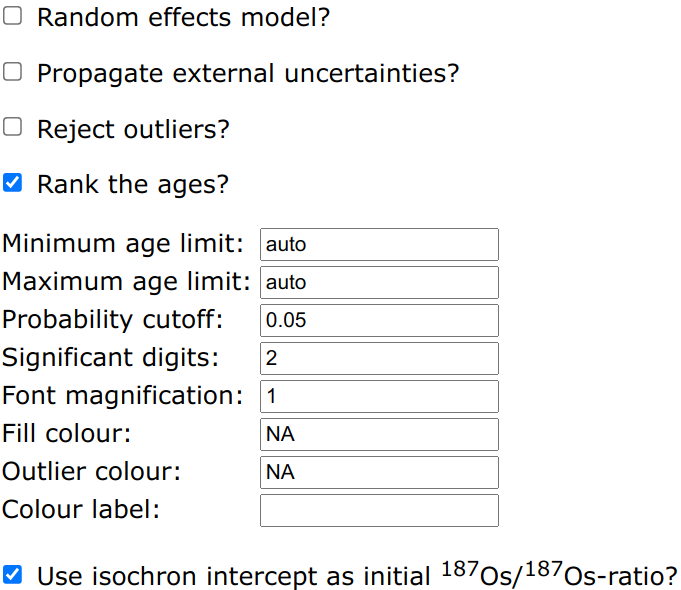
\includegraphics[width=\linewidth]{../figures/ReOsWtdMean.png}
\end{minipage}
\begin{minipage}[t]{.45\linewidth}
  The settings shown here implement the ordinary weighted mean of
  Re--Os data whose non-radiogenic Os-composition is obtained from an
  isochron fit. Decay constants have been omitted from the weighted
  mean age, and the aliquots are not filtered by the modified
  Chauvenet outlier detection algorithm. Aliquots are ranked according
  to age. The plot uses the default y-axis limits, significance
  criterion, precision and font size. Aliquots are plotted as empty
  rectangles.
\end{minipage}

\begin{console}
weightedmean(ReOs,detect.outliers=FALSE,ranked=TRUE,rect.col=NA,i2i=TRUE)
\end{console}

\item\noindent\begin{minipage}[t]{.55\linewidth}
\strut\vspace*{-\baselineskip}\newline
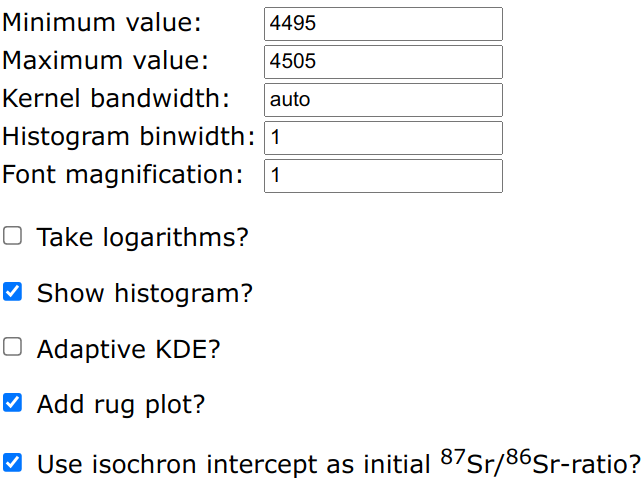
\includegraphics[width=\linewidth]{../figures/RbSrKDE.png}
\end{minipage}
\begin{minipage}[t]{.45\linewidth}
  The settings here create a KDE of Rb--Sr data that ranges from 4495
  to 4505~Ma, uses a fixed but default \citet{botev2010} histogram
  bandwidth and a 1~Myr histogram bin width. The non-radiogenic
  Sr-composition is derived from the best fitting isochron intercept.
  All other settings follow the default values.
\end{minipage}

\begin{console}
cad(RbSr,from=4495,to=4505,binwidth=1,adaptive=FALSE,i2i=TRUE)
\end{console}

\item\noindent\begin{minipage}[t]{.65\linewidth}
\strut\vspace*{-\baselineskip}\newline
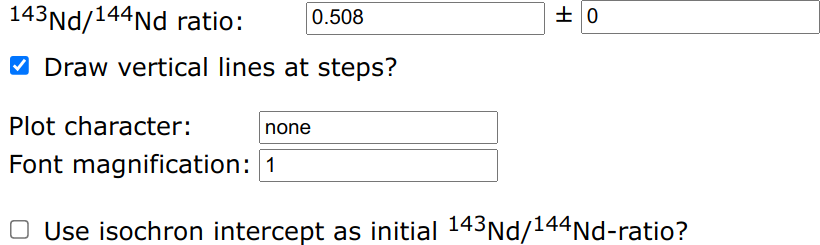
\includegraphics[width=\linewidth]{../figures/SmNdCAD.png}
\end{minipage}
\begin{minipage}[t]{.35\linewidth}
  Settings for a CAD plot of Sm--Nd data with a nominal inherited
  \textsuperscript{142}Nd/\textsuperscript{144}Nd-ratio of 0.508
  and default values for all other settings.
\end{minipage}

\begin{console}
settings('iratio','Nd143Nd144',0.508)
cad(SmNd,i2i=FALSE)
\end{console}

\end{enumerate}

\printbibliography[heading=subbibliography]

\end{refsection}
